\documentclass[a4paper,10pt]{article}
\usepackage[utf8]{inputenc}
\usepackage[margin=1.5cm, bottom=2cm]{geometry}
\usepackage{fancyhdr}
\usepackage{enumitem}
\usepackage{xcolor}
\usepackage[most]{tcolorbox}
\newtcolorbox{osservazioni}{
  colback=gray!8,    % sfondo grigio chiaro
  colframe=white,      % nessun bordo
  arc=2mm,            % angoli smussati
  boxrule=0pt,        % spessore bordo 0
  fontupper=\footnotesize,
  left=2mm, right=2mm, top=2mm, bottom=2mm,
  before skip=7pt,   % niente spazio prima
  after skip=15pt     % niente spazio dopo
}
\pagestyle{fancy}
\usepackage{tikz}
\usetikzlibrary{automata, positioning}
\pagestyle{fancy}


%%%%%%%%%%%%%%%%%%%
\newcommand{\EsercitazioneNum}{03}
\newcommand{\Data}{09/09/2025}
%%%%%%%%%%%%%%%%%%%

% Numero di pagina in basso al centro
\fancyhf{}
\fancyfoot[C] \thepage
\renewcommand{\footrulewidth}{0pt} % niente linea in basso
\renewcommand{\headrulewidth}{0pt} % niente linea in alto

\begin{document}
\footnotesize  % font generale più piccolo

\noindent
\small \textbf{Computabilità, Complessità e Logica - a.a. 2025/26} \hfill \textbf{Esercitazione \EsercitazioneNum} \\[0.2cm]
\scriptsize Matteo Liotta, \texttt{matteo.liotta@studenti.units.it} \hfill \Data \\[0.2cm]

\noindent\makebox[\linewidth]{\rule{\linewidth}{0.4pt}} \\[1cm]


\noindent\Large \textbf{Esercitazione \EsercitazioneNum}: \textit{Operazioni di chiusura per Automi Regolari}
\begin{osservazioni}
    \textbf{\textit{Nota}}. Sono indicati in \textcolor{blue}{\textit{blu}} gli esercizi che non saranno trattati durante l'esercitazione, bensì lasciati come strumento aggiuntivo di esercitazione individuale. Resta comunque assoluta disponibilità per la loro risoluzione negli incontri successivi, qualora necessario.
\end{osservazioni}

{\normalsize
\begin{itemize}[label=, leftmargin=0pt]

\item\underline{\textit{\textbf{Determinizzazione di Automi Regolari ND}}}
    
    \item \textbf{Esercizio 1. (*)}\\ 
    Dato il seguente automa regolare non deterministico definito su $\Sigma=\{a,b\}$, se ne rappresenti graficamente la determinizzazione.
    {
    \small
    \begin{center}
    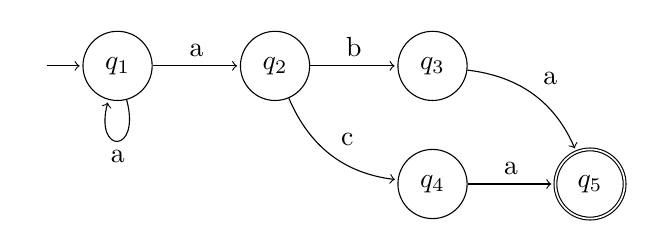
\begin{tikzpicture}[shorten >=1pt, node distance=2cm, on grid, auto]
        \node[state, initial, initial text=] (q1)   {$q_1$};
        \node[state] (q2) [right=of q1] {$q_2$};
        \node[state] (q3) [right=of q2] {$q_3$};
        \node[state] (q4) [below=1.5 of q3] {$q_4$};
        \node[state, accepting] (q5) [right=of q4] {$q_5$};
        
        \path[->]
        (q1) edge [loop below] node {a} (q1)
             edge node {a} (q2)
        (q2) edge node {b} (q3)
             edge [bend right] node {c} (q4)
        (q3) edge [bend left] node {a} (q5)
        (q4) edge node {a} (q5);
    \end{tikzpicture}
    \end{center}
    }%\\[0.1cm]



    \item \textcolor{blue}{\textbf{Esercizio 2. (*)} }\\ 
    Dato il seguente automa regolare non deterministico definito su $\Sigma=\{a\}$, se ne rappresenti graficamente la determinizzazione.
    {
    \small
    \begin{center}
    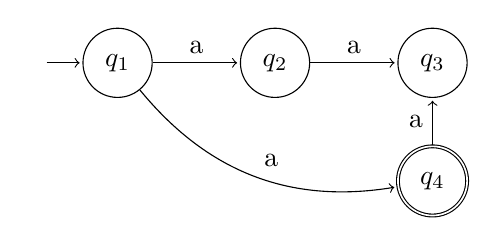
\begin{tikzpicture}[shorten >=1pt, node distance=2cm, on grid, auto]
        \node[state, initial, initial text=] (q1)   {$q_1$};
        \node[state] (q2) [right=of q1] {$q_2$};
        \node[state] (q3) [right=of q2] {$q_3$};
        \node[state, accepting] (q4) [below=1.5 of q3] {$q_4$};
        
        \path[->]
        (q1) edge node {a} (q2)
             edge [bend right] node {a} (q4)
        (q2) edge node {a} (q3)
        (q4) edge node {a} (q3);
        
             
    \end{tikzpicture}
    \end{center}
    }


    \item \textbf{Esercizio 3. (**)}\\ 
    Dato il seguente automa regolare non deterministico definito su $\Sigma=\{a,b,c\}$, se ne rappresenti graficamente la determinizzazione.
    {
    \small
    \begin{center}
    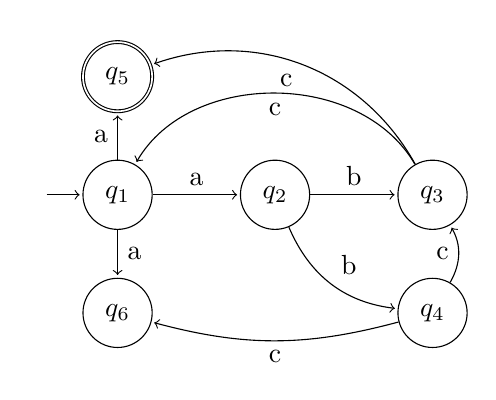
\begin{tikzpicture}[shorten >=1pt, node distance=2cm, on grid, auto]
        \node[state, initial, initial text=] (q1)   {$q_1$};
        \node[state] (q2) [right=of q1] {$q_2$};
        \node[state] (q3) [right=of q2] {$q_3$};
        \node[state] (q4) [below=1.5 of q3] {$q_4$};
        \node[state, accepting] (q5) [above=1.5of q1] {$q_5$};
        \node[state] (q6) [below=1.5of q1] {$q_6$};
        
        \path[->]
        (q1) edge node {a} (q2)
             edge node {a} (q6)
             edge node {a} (q5)
        (q2) edge node {b} (q3)
             edge [bend right] node {b} (q4)
        (q4) edge [bend left=15] node {c} (q6)
             edge [bend right] node {c} (q3)
        (q3) edge [bend right=60] node {c} (q1)
             edge [bend right=40] node {c} (q5);
             
    \end{tikzpicture}
    \end{center}
    }
    $\\$
\item \underline{\textit{\textbf{Complementazione di Automi Regolari}}}

    
    \item \textbf{Esercizio 4. (*)}\\ 
    Dato il seguente automa regolare definito su $\Sigma=\{a,b\}$. Si rappresenti graficamente l'automa che accetti il linguaggio regolare complementare:
    
    {
    \small
    \begin{center}
    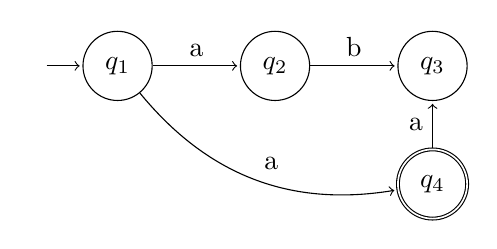
\begin{tikzpicture}[shorten >=1pt, node distance=2cm, on grid, auto]
        \node[state, initial, initial text=] (q1)   {$q_1$};
        \node[state] (q2) [right=of q1] {$q_2$};
        \node[state] (q3) [right=of q2] {$q_3$};
        \node[state, accepting] (q4) [below=1.5 of q3] {$q_4$};
        
        \path[->]
        (q1) edge node {a} (q2)
             edge [bend right] node {a} (q4)
        (q2) edge node {b} (q3)
        (q4) edge node {a} (q3);
        
             
    \end{tikzpicture}
    \end{center}
    }

    \vfill
    \noindent\makebox[\linewidth]{\rule{\linewidth}{0.4pt}}
    \newpage
    {\noindent
    \small \textbf{Computabilità, Complessità e Logica - a.a. 2025/26} \hfill \textbf{Esercitazione \EsercitazioneNum} \\[0.2cm]
    \scriptsize Matteo Liotta, \texttt{matteo.liotta@studenti.units.it} \hfill \Data \\[0.2cm]
    \noindent\makebox[\linewidth]{\rule{\linewidth}{0.4pt}} \\[0.3cm]}

    


    \item \textbf{Esercizio 5. (***)}\\ 
    Dato il seguente automa regolare definito su $\Sigma=\{a,b\}$. Si rappresenti graficamente l'automa che accetti il linguaggio regolare complementare.
    {
    \small
    \begin{center}
    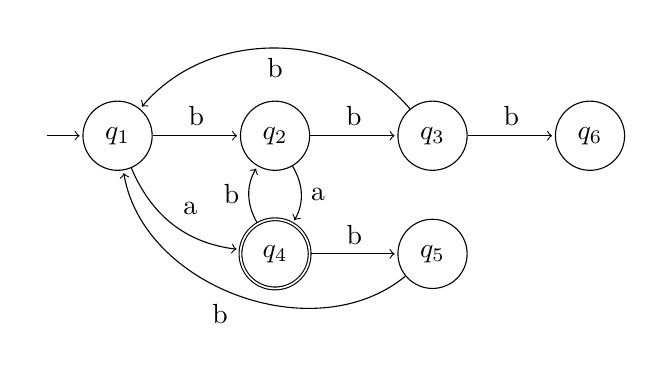
\begin{tikzpicture}[shorten >=1pt, node distance=2cm, on grid, auto]
        \node[state, initial, initial text=] (q1)   {$q_1$};
        \node[state] (q2) [right=of q1] {$q_2$};
        \node[state] (q3) [right=of q2] {$q_3$};
        \node[state, accepting] (q4) [below=1.5 of q2] {$q_4$};
        \node[state] (q5) [below=1.5 of q3] {$q_5$};
        \node[state] (q6) [right=of q3] {$q_6$};

        \path[->]
        (q1) edge node {b} (q2)
             edge [bend right] node {a} (q4)
        (q2) edge node {b} (q3)
             edge [bend left] node {a} (q4)
        (q3) edge node {b} (q6)
             edge [bend right=50] node {b} (q1)
        (q4) edge [bend left] node {b} (q2)
             edge node {b} (q5)
        (q5) edge [bend left=60] node {b} (q1);
        
             
    \end{tikzpicture}
    \end{center}
    }
    
\item \textcolor{blue}{\textbf{Esercizio 6. (*) }\\ }
    Dato il seguente automa regolare definito su $\Sigma=\{a,b,c\}$. Si rappresenti graficamente l'automa che accetti il linguaggio regolare complementare.
    {
    \small
    \begin{center}
    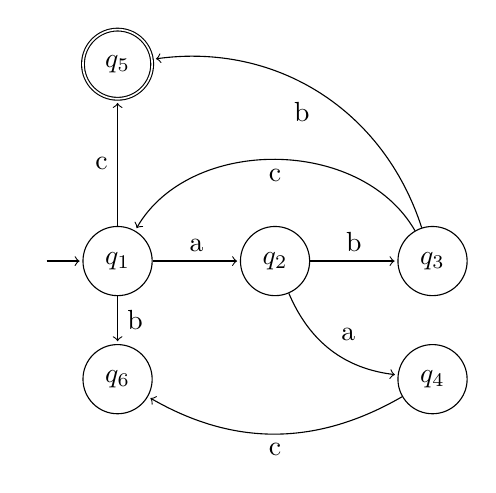
\begin{tikzpicture}[shorten >=1pt, node distance=2cm, on grid, auto]
        \node[state, initial, initial text=] (q1)   {$q_1$};
        \node[state] (q2) [right=of q1] {$q_2$};
        \node[state] (q3) [right=of q2] {$q_3$};
        \node[state] (q4) [below=1.5 of q3] {$q_4$};
        \node[state, accepting] (q5) [above=2.5of q1] {$q_5$};
        \node[state] (q6) [below=1.5of q1] {$q_6$};
        
        \path[->]
        (q1) edge node {a} (q2)
             edge node {b} (q6)
             edge node {c} (q5)
        (q2) edge node {b} (q3)
             edge [bend right] node {a} (q4)
        (q4) edge [bend left] node {c} (q6)
        (q3) edge [bend right=60] node {c} (q1)
             edge [bend right=40] node {b} (q5);
 
    \end{tikzpicture}
    \end{center}
    }

    \item \textbf{Esercizio 7. (***)}\\ 
    Sia $L$ linguaggio regolare su $\Sigma =\{a,b\}$, tale per cui
    {\begin{center}
        $L = \{ w \in \Sigma^* \mid w\ \text{ha\ un\ numero\ pari\ di\ a\ e\ multiplo\ di\ 3\ di\ b}\}$
    \end{center}} 
    Si rappresenti graficamente l'automa l'automa che riconosca il linguaggio ad esso complementare.
    $\\\\$
    

    \item \underline{\textit{\textbf{Unione di Automi Regolari}}}

    \item \textbf{Esercizio 8. (**)}\\ 
    Siano $L_1, L_2$ linguaggi regolare su $\Sigma =\{a,b\}$, tali per cui
    {
    \begin{enumerate}
        \item $L_1 = \{ w \in \Sigma^* \mid w\ \text{ha\ un\ numero\ pari\ di\ a}\}$\\
        \item $L_2 = \{ w \in \Sigma^* \mid w\ \text{ha\ un\ numero\ multiplo di 3\ di\ b}\}$
    \end{enumerate}
    } 
    Si rappresentino graficamente gli automi che riconoscono il linguaggio $L_1,L_2$ e da essi si ricavi l'automa unione, preservando il determinismo.
    

    \vfill
    \noindent\makebox[\linewidth]{\rule{\linewidth}{0.4pt}}
    \newpage
    {\noindent
    \small \textbf{Computabilità, Complessità e Logica - a.a. 2025/26} \hfill \textbf{Esercitazione \EsercitazioneNum} \\[0.2cm]
    \scriptsize Matteo Liotta, \texttt{matteo.liotta@studenti.units.it} \hfill \Data \\[0.2cm]
    \noindent\makebox[\linewidth]{\rule{\linewidth}{0.4pt}} \\[0.3cm]}


    \item \textcolor{blue}{\textbf{Esercizio 9. (**)}}\\ 
    Sia $L$ linguaggio regolare su $\Sigma =\{a,b\}$, tale per cui
    {\begin{center}
    $L = \{ w \in \Sigma^* \mid w = a^nb^2, n\geq 0\}$\\
    \end{center}}
    Si rappresentino graficamente gli automi che riconoscono il linguaggio $L$ ed $\overline{L}$ e da essi si ricavi l'automa unione; si mostri per tale automa l'accettazione di $\Sigma^*$.

    $\\$
    \item \underline{\textit{\textbf{Intersezione di Automi Regolari}}}

    
    \item \textbf{Esercizio 10. (*)}\\ 
    Si conisderino nuovamente (cfr. es. 9) $L, \overline{L}$, linguaggi regolari su $\Sigma =\{a,b\}$, tali per cui
    {\begin{center}
    $L = \{ w \in \Sigma^* \mid w = a^nb^2, n\geq 0\}$\\
    \end{center}}
    Si rappresenti allora graficamente l'automa prodotto tale da riconoscere l'intersezione dei linguaggi. Quale linguaggio è dunque riconosciuto da tale automa?


\item {\textbf{Esercizio 11. (***)}\\ 
    Dati i due automi dei precedenti esercizi, definiti rispettivamente sui linguaggi $\Sigma_1$ e $\Sigma_2$:
    {
    \small
    \begin{center}
    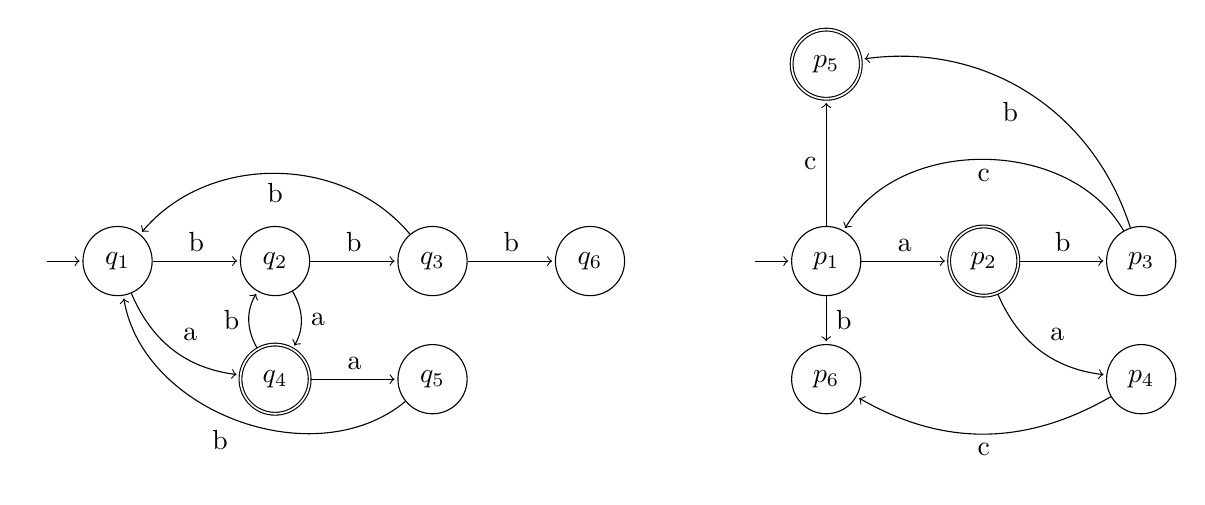
\begin{tikzpicture}[shorten >=1pt, node distance=2cm, on grid, auto]
        \node[state, initial, initial text=] (q1)   {$q_1$};
        \node[state] (q2) [right=of q1] {$q_2$};
        \node[state] (q3) [right=of q2] {$q_3$};
        \node[state, accepting] (q4) [below=1.5 of q2] {$q_4$};
        \node[state] (q5) [below=1.5 of q3] {$q_5$};
        \node[state] (q6) [right=of q3] {$q_6$};

        \path[->]
        (q1) edge node {b} (q2)
             edge [bend right] node {a} (q4)
        (q2) edge node {b} (q3)
             edge [bend left] node {a} (q4)
        (q3) edge node {b} (q6)
             edge [bend right=50] node {b} (q1)
        (q4) edge [bend left] node {b} (q2)
             edge node {a} (q5)
        (q5) edge [bend left=60] node {b} (q1);

        \node[state, initial, initial text=, right=3of q6] (p1)   {$p_1$};
        \node[state, accepting] (p2) [right=of p1] {$p_2$};
        \node[state] (p3) [right=of p2] {$p_3$};
        \node[state] (p4) [below=1.5 of p3] {$p_4$};
        \node[state, accepting] (p5) [above=2.5of p1] {$p_5$};
        \node[state] (p6) [below=1.5of p1] {$p_6$};
        
        \path[->]
        (p1) edge node {a} (p2)
             edge node {b} (p6)
             edge node {c} (p5)
        (p2) edge node {b} (p3)
             edge [bend right] node {a} (p4)
        (p4) edge [bend left] node {c} (p6)
        (p3) edge [bend right=60] node {c} (p1)
             edge [bend right=40] node {b} (p5);
 
    \end{tikzpicture}
    \end{center}
    }
    Si rappresenti graficamente l'automa prodotto, tale da accettare l'intersezione dei linguaggi riconosciuti rispettivamente da ciascun automa.

    \textcolor{blue}{\item \textbf{Esercizio 12. (*)} \\ }
    Si conisderino nuovamente (cfr. es. 9) $L, \overline{L}$, linguaggi regolari su $\Sigma =\{a,b\}$, tali per cui
    {
    \begin{center}
    $L = \{ w \in \Sigma^* \mid w = a^nb^2, n\geq 0\}$\\
    \end{center}
    }
    Si rappresenti allora graficamente l'automa prodotto tale da riconoscere l'intersezione dei linguaggi. Quale linguaggio è dunque riconosciuto da tale automa?

    
\end{itemize}
}
\vfill
\noindent\makebox[\linewidth]{\rule{\linewidth}{0.1pt}}
\end{document}
